% chktex-file 24
\chapter{Descrizione dello stage}
\label{cap:descrizione-stage}

\emph{In questo capitolo viene presentata una panoramica del progetto di stage, con una descrizione dettagliata del contesto aziendale, del progetto e degli obiettivi prefissati. Vengono inoltre elencati i requisiti e gli obiettivi del progetto, i prodotti attesi e la pianificazione delle attività.}

\section{Introduzione al progetto}

Le organizzazioni di diversi settori, come sanità, finanza, legale, retail e manifatturiero, gestiscono quotidianamente una grande quantità di documenti nei loro processi aziendali. Questi documenti contengono informazioni critiche, essenziali per prendere decisioni tempestive e mantenere alti livelli di soddisfazione del cliente, velocizzare l'onboarding e ridurre il tasso di abbandono dei clienti. Nella maggior parte dei casi, l'elaborazione di tali documenti avviene manualmente, un processo che richiede tempo, è soggetto a errori, costoso e difficile da scalare. Inoltre, l'automazione attualmente disponibile per l'elaborazione dei documenti è limitata.

L'elaborazione intelligente dei documenti (\glsfirstoccur{\gls{idp}}) consente di automatizzare l'estrazione delle informazioni da documenti di diverso tipo e formato, in modo rapido e preciso, senza necessità di competenze avanzate di \glsfirstoccur{\gls{machinelearningg}}. Questa tecnologia riduce i costi complessivi, migliorando al contempo l'efficienza e la qualità delle decisioni aziendali.

\gls{idpg} automatizza la raccolta e l'elaborazione delle informazioni dai documenti digitali o cartacei, integrandole nei flussi di lavoro aziendali digitali. Ad esempio, in un'azienda che invia ordini ai fornitori al calo delle scorte, \gls{idpg} sostituisce l'immissione manuale dei dati estraendo automaticamente le informazioni rilevanti dalle fatture ricevute via e-mail e integrandole nel sistema contabile. Questo processo elimina gli ostacoli e riduce notevolmente gli errori, migliorando l'efficienza operativa.

\gls{idpg} offre numerosi vantaggi alle aziende, come la \glsfirstoccur{\gls{scalabilitàg}} nella gestione di grandi volumi di documenti, l'automazione delle attività ripetitive e la riduzione dei costi di elaborazione manuale. Inoltre, velocizza l'interazione con i clienti, automatizzando attività come l'onboarding e la gestione dei pagamenti, garantendo risposte tempestive e personalizzate. 

I settori che beneficiano dell'\gls{idpg} includono la sanità, dove facilita la gestione delle cartelle cliniche e l'organizzazione dei dati medici; le finanze, dove automatizza la gestione delle spese e delle fatture; il settore legale, dove analizza contratti e documenti complessi; la logistica, dove migliora la tracciabilità delle spedizioni; e le risorse umane, dove semplifica la selezione del personale e gestisce le buste paga.

Le tecnologie principali che supportano l'\gls{idpg} includono il riconoscimento ottico dei caratteri (\glsfirstoccur{\gls{ocr}}), che converte le immagini di testo in dati leggibili dalle macchine, e l'elaborazione del linguaggio naturale (\glsfirstoccur{\gls{nlp}}), che analizza e comprende il linguaggio umano. L'automazione robotica dei processi (\glsfirstoccur{\gls{rpa}}) permette di ripetere azioni umane predefinite per automatizzare i flussi di lavoro aziendali.

Il processo di \gls{idpg} (vedi Figura~\ref{fig:idp_workflow}) segue tipicamente diverse fasi: acquisizione e classificazione dei documenti, estrazione dei dati tramite \gls{ocrg} e \gls{nlpg}, convalida e inserimento delle informazioni nei sistemi aziendali, e apprendimento continuo attraverso modelli di \gls{machinelearningg} per migliorare l'accuratezza. I sistemi di \gls{idpg} forniscono anche report e analisi che aiutano le aziende a ottimizzare ulteriormente i loro flussi di lavoro.

In un contesto aziendale sempre più orientato all'innovazione, l'elaborazione dei documenti ha subito notevoli trasformazioni grazie all'introduzione dell'\gls{idpg}, che trasforma i dati non strutturati presenti in vari tipi di documenti in informazioni strutturate e fruibili, migliorando drasticamente l'efficienza e riducendo lo sforzo manuale. Tuttavia, il potenziale dell'\gls{idpg} non si esaurisce qui. Con l'integrazione dell'intelligenza artificiale generativa (\glsfirstoccur{\gls{generativeaig}}), l'\gls{idpg} può essere ulteriormente potenziata.

L'integrazione di modelli di linguaggio di grandi dimensioni (\glsfirstoccur{\gls{llmg}}) nelle architetture \gls{idpg} consente di ottenere capacità avanzate di estrazione dati, adattandosi dinamicamente ai cambiamenti nei modelli dei dati. Amazon Web Services \gls{awsg} supporta questa evoluzione con strumenti come Amazon Textract, un servizio di machine learning (\gls{machinelearningg}) che estrae automaticamente testo, scrittura e dati da documenti scansionati, e Amazon Bedrock, un servizio completamente gestito che offre modelli di intelligenza artificiale di base attraverso \glsfirstoccur{\gls{apig}} di facile utilizzo. Un ulteriore strumento chiave è Amazon Comprehend, un servizio di \gls{nlpg} che consente di analizzare e comprendere il contenuto dei documenti, estraendo informazioni chiave, come entità, sentiment e concetti, direttamente dal testo.

In particolare, l'integrazione di Amazon Textract con LangChain, utilizzato come document loader, e Amazon Bedrock, per l'estrazione di dati e capacità di \gls{aig}, permette di estendere le funzionalità di una nuova o esistente architettura \gls{idpg}. Amazon Comprehend si combina perfettamente in questo flusso, utilizzando \gls{nlpg} per analizzare il contenuto dei documenti e fornire insight dettagliati, aumentando la precisione dell'estrazione delle informazioni e permettendo di ottenere analisi più approfondite.

Questa combinazione introduce non solo un'automazione più avanzata nell'elaborazione dei documenti, ma anche una capacità di adattamento e miglioramento continuo grazie all'\gls{aig}, consentendo di affrontare in modo dinamico i modelli di dati in evoluzione.

In conclusione, l'integrazione di \gls{idpg}, \gls{aig} e strumenti come Amazon Textract, Amazon Comprehend e Amazon Bedrock rappresenta una nuova frontiera nell'elaborazione documentale, offrendo alle aziende non solo efficienza operativa, ma anche flessibilità e capacità di risposta alle nuove sfide del mercato.

Nel contesto del progetto di stage, l'obiettivo è implementare un modello di \gls{aig} per l'elaborazione intelligente degli allegati delle \gls{pecg} e per perseguire a questo scopo, si è deciso di utilizzare i servizi \gls{awsg} per l'addestramento del modello di \gls{aig} e per l'elaborazione delle \gls{pecg} importate. 

\begin{figure}[!ht]
    \centering
    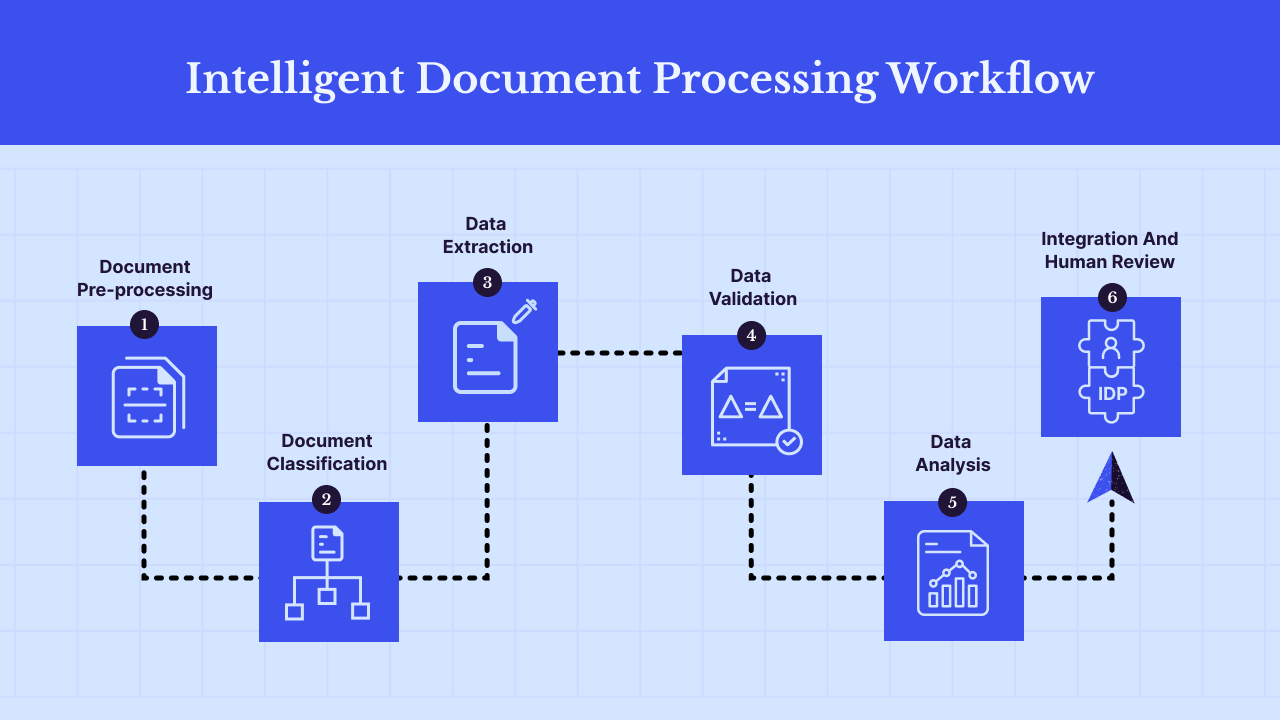
\includegraphics[width=0.8\columnwidth]{idp_workflow.png}
    \caption{Flusso di lavoro dell'elaborazione intelligente dei documenti}
    \label{fig:idp_workflow}
\end{figure}



%\begin{figure}[!ht]
%    \centering
%    \includegraphics[width=0.5\columnwidth]{pk_estate.jpg}
%    \caption{Caption}
%\end{figure}
%Digressione su idp.\\
%\lipsum[1]

%\section{Analisi preventiva dei rischi}
%
%Durante la fase di analisi iniziale sono stati individuati alcuni possibili
%rischi a cui si potrà andare incontro. Si è quindi proceduto a elaborare delle
%possibili soluzioni per far fronte a tali rischi.
%
%\begin{risk}{Performance del simulatore hardware}
%    \riskdescription{le performance del simulatore hardware e la comunicazione con questo potrebbero risultare lenti o non abbastanza buoni da causare il fallimento dei test}
%    \risksolution{coinvolgimento del responsabile a capo del progetto relativo il simulatore hardware}
%    \label{risk:hardware-simulator}
%\end{risk}
%
\section{Requisiti e obiettivi}

Gli obiettivi del progetto sono stati definiti in accordo con il tutor aziendale e si articolano nel modo seguente:
\[
    \text{[Priorità][Id]}
\]
\begin{itemize}
    \item \textbf{Priorità}: indica il livello di importanza dell'obiettivo, che può essere \emph{Obbligatorio} o \emph{Desiderabile};
    \item \textbf{Id}: composto da due cifre, identifica in modo univoco l'obiettivo rispetto alla priorità.
\end{itemize}

Di seguito è riportata una tabella che elenca i requisiti e gli obiettivi stabiliti per il progetto.

\begin{longtable}{|c|p{4cm}|p{10cm}|}
    \hline
    \textbf{ID}  & \textbf{Categoria}                                               & \textbf{Descrizione}                                       \\
    \hline
    \endfirsthead

    \hline
    \textbf{ID}  & \textbf{Categoria}                                               & \textbf{Descrizione}                                       \\
    \hline
    \endhead

    O01          & Obbligatorio                                                     & Analisi dei servizi \gls{awsg} per l'addestramento dei modelli di \gls{aig}. \\
    \hline 
    O02          & Obbligatorio                                                     & Addestramento di un modello di apprendimento \gls{aig} utilizzando i servizi \gls{awsg}. \\
    \hline 
    O03          & Obbligatorio                                                     & Analisi dei requisiti applicativi e tecnici per implementare la soluzione richiesta. \\
    \hline 
    O04          & Obbligatorio                                                     & Implementazione di un modello di apprendimento automatico che analizzi il contenuto delle \gls{pecg} importate e assegni loro categorie appropriate (mittente, destinatario, data e argomento). \\
    \hline 
    D01          & Desiderabile                                                     & Implementazione di algoritmi di \gls{aig} in grado di adattarsi e apprendere continuamente dai dati per migliorare le prestazioni del sistema nel tempo. Questo include l'ottimizzazione dei modelli di apprendimento in base all'esperienza e ai feedback degli utenti. \\
    \hline 
    D02          & Desiderabile                                                     & Integrazione con un sistema documentale per l'archiviazione delle \gls{pecg}, creando i metadati necessari e assegnando le informazioni estratte alla corretta categoria. \\
    \hline
    \caption{Tabella dei requisiti e obiettivi dello stage} \\
\end{longtable}

\subsection{Prodotti attesi}

Tra i principali risultati attesi dal progetto, lo studente dovrà produrre una relazione scritta che illustri in dettaglio i punti chiave del lavoro svolto. In particolare, la relazione dovrà includere:

\begin{itemize}
    \item Una contestualizzazione del progetto, che spieghi il problema affrontato e gli obiettivi perseguiti;
    \item Un'analisi completa e approfondita che copra:
    \begin{itemize}
        \item L'inquadramento generale del progetto;
        \item I requisiti applicativi e tecnici;
        \item La struttura del database;
        \item Gli strumenti e le applicazioni di terze parti utilizzati;
        \item I principali casi d'uso individuati.
    \end{itemize}
    \item Uno studio di fattibilità, volto a dimostrare la possibilità di implementare la soluzione proposta;
    \item La descrizione dettagliata dell'implementazione della soluzione sviluppata.
\end{itemize}

\subsection{Contenuti formativi previsti}

Nel corso di questo progetto di stage, lo studente avrà l'opportunità di approfondire diverse aree tecniche e migliorare le proprie competenze. In particolare, gli ambiti di conoscenza che saranno oggetto di apprendimento includono:

\begin{itemize}
    \item \textbf{Linguaggi e strumenti tecnologici}: lo studente acquisirà familiarità con una serie di tecnologie chiave, tra cui:
    \begin{itemize}
        \item L'uso del database MySQL, se necessario per il progetto;
        \item I framework più diffusi come Angular, Maven, Spring e \gls{awsg} \glsfirstoccur{\gls{sdkg}};
        \item Diversi linguaggi di programmazione e formati di dati, quali Java, JSON, HTML, CSS, Javascript, Typescript e il formato PDF/A2;
        \item I servizi cloud di \gls{awsg}, utilizzati per l'addestramento dei modelli di \gls{ai};
        \item Python e gli strumenti di analisi forniti da notebook Jupyter.
    \end{itemize}
    \item \textbf{Competenze trasversali}: lo studente acquisirà inoltre esperienza pratica nel lavoro di gruppo, in particolare all'interno di un team che utilizza il framework \gls{agileg} \gls{scrumg}, migliorando così le proprie capacità di collaborazione e gestione del lavoro in un contesto aziendale strutturato.
\end{itemize}

\section{Pianificazione}

La pianificazione delle attività è stata organizzata in base agli obiettivi prefissati e alle scadenze stabilite. La tabella seguente riporta la pianificazione settimanale delle attività svolte durante il periodo di stage.

\begin{longtable}{|c|c|c|p{8cm}|}
    \hline
    \textbf{Settimana} & \textbf{Dal} & \textbf{Al} & \textbf{Attività}                                          \\
    \hline
    \endfirsthead

    \hline
    \textbf{Settimana} & \textbf{Dal} & \textbf{Al} & \textbf{Attività}                                          \\
    \hline
    \endhead

    1                  & 24-06-2024   & 28-06-2024  &
    Incontro con le persone coinvolte nel progetto per discutere i requisiti e le richieste di implementazione; ricerca, studio e documentazione per l'inquadramento del progetto; introduzione ai linguaggi di sviluppo; introduzione agli ambienti di sviluppo; introduzione dei servizi \gls{awsg}. \\
    \hline
    2                  & 01-07-2024   & 05-07-2024  &
    Analisi dei servizi \gls{awsg} per l'addestramento di un modello di apprendimento; addestramento di un modello di apprendimento utilizzando i servizi di \gls{awsg}. \newline \textbf{Milestone:} Utilizzo dei servizi \gls{awsg} per l'addestramento di un modello di apprendimento. \\
    \hline
    3                  & 08-07-2024   & 12-07-2024  &
    Studio della soluzione per definire i requisiti necessari per l’implementazione. \newline \textbf{Milestone:} Analisi dei requisiti applicativi e tecnici per implementare la soluzione. \\
    \hline
    4                  & 15-07-2024   & 19-07-2024  &
    Addestramento del modello di apprendimento per catalogare le \gls{pecg} in base al loro contenuto. \\
    \hline
    5                  & 22-07-2024   & 26-07-2024  &
    Implementazione per interfacciarsi con il modello di apprendimento addestrato e per catalogare le \gls{pecg} importate.\newline \textbf{Milestone:} Completamento degli obiettivi minimi. \\
    \hline
    6                  & 29-07-2024   & 02-08-2024  &
    Implementazione dell'algoritmo di \gls{aig} per l’autoapprendimento. \\
    \hline
    7                  & 05-08-2024   & 09-08-2024  &
    Studio e documentazione sulle \glsfirstoccur{\gls{apig}} messe a disposizione dal sistema documentale per catalogare le mail \gls{pecg}; implementazione dell’integrazione con il documentale producendo i metadati necessari per catalogare le \gls{pecg}. \\
    \hline
    8                  & 12-08-2024   & 16-08-2024  &
    Verifica e test dell'archiviazione delle \gls{pecg} nel documentale.\newline \textbf{Milestone:} Completamento degli obiettivi massimi. \\
    \hline
    9                  & 19-08-2024   & 23-08-2024  &
    Recupero di eventuali ritardi. \\
    \hline
    10                 & 26-08-2024   & 30-08-2024  &
    Recupero di eventuali ritardi. \\
    \hline
    \caption{Tabella della pianificazione dello stage} \\
\end{longtable}

Durante lo svolgimento dello stage, sono state applicate modifiche alla pianificazione in base alle necessità e alle richieste del tutor aziendale.

\section{Organizzazione del lavoro}

Lo stage si è svolto nel periodo dal 24 giugno 2024 al 30 agosto 2024, con una durata complessiva di 8 settimane e un totale di 320 ore di lavoro. È stata prevista una modalità mista, con 2 giorni a settimana di presenza in azienda e 3 giorni in modalità remota, con impegno full-time ogni giorno. La sede di riferimento è stata quella di \myCompany situata in Via dell'Edilizia, 100, Vicenza (VI), ovvero il Centro per la Formazione.

Lo studente è stato inserito in un gruppo di lavoro, con il supporto continuo del team e del tutor aziendale. Il tutor è stato spesso presente nel gruppo, garantendo una modalità di interazione costante e facilitando il processo di revisione e feedback. Le revisioni del progetto sono state condotte in conformità alla metodologia \gls{scrumg}, con brevi riunioni giornaliere di 5 minuti e una revisione settimanale della durata di 1 ora.

L'azienda ha fornito strumenti di comunicazione e collaborazione come \emph{Google Meet} per le riunioni e \emph{Google Drive} per la condivisione dei documenti, organizzati attraverso un gruppo creato su Gmail. La comunicazione in modalità smart working è avvenuta tramite la chat di \emph{Google Chat}, garantendo un canale diretto per il dialogo tra lo studente e il tutor aziendale.

Oltre ai punti sopra elencati, durante il corso dello stage sono stati svolti due incontri con il tutor aziendale, denominati SAL (Stato Avanzamento Lavoro), per discutere lo stato di avanzamento del progetto e valutare eventuali modifiche da apportare. Il primo incontro è stato svolto a metà stage, mentre il secondo è avvenuto alla conclusione dello stage. L'incontro di chiusura è stato utilizzato per discutere i risultati ottenuti e per valutare il lavoro complessivo svolto.